%\documentclass[12pt,a4]{article}

%\title{Part II Project Proposal: Functional Reactive Programming for Data Binding in C$\sharp$ }
%\author{David Barker\\Project supervisor: Tomas Petricek}

%\usepackage{fullpage}
%\usepackage{listing}
%\usepackage{graphicx}

%\begin{document}

%\maketitle

\vfil

\centerline{\Large Part II Project Proposal}
\vspace{0.4in}
\centerline{\Large Functional Reactive Programming for Data Binding in C$\sharp$\ }
\vspace{0.4in}
\centerline{\large David Barker, Jesus College}
\vspace{0.3in}
\centerline{\large Originator: Tomas Petricek}
\vspace{0.3in}
\centerline{\large \today}

\vfil


\noindent
{\bf Project Supervisor:} Tomas Petricek
\vspace{0.2in}

\noindent
{\bf Director of Studies:} Prof. Jean Bacon
\vspace{0.2in}
\noindent

\section*{Introduction and Description of the Work}

	Data binding is widely used throughout software design as a general way of linking two properties together such that their values are synchronised. This is useful in many areas -- for instance, in user interface programming, data binding can be used to allow the interface to directly reflect the underlying model with minimal code on its part. As a result, data binding is now a standard feature in some widely-used languages and frameworks.\footnote{For instance, Javascript\cite{javabinding} and .NET\cite{netbinding} both provide this functionality} However, it is often fairly limited in that only direct bindings are available (where the destination's value is exactly that of the source) and they generally only work in one direction.
	
	A feature some frameworks provide is \textit{functional} data binding. This is where the value of a binding source is passed through a function to the binding destination,\footnote{Microsoft Excel's formula cells are a widely-used example of this} and so a more complex binding can be established. This works well for many applications, but is still not as natural to use as it could be. It also still suffers from the limitation of only working in one direction, which prevents the programmer from having two mutable properties which are functionally linked.
	
	One way of making this idea of functional data binding more general is through functional reactive programming (FRP). This is a paradigm in which behaviour is defined \textit{reactively} on input signals which can vary either discretely or continuously. Elliott\cite{elliott98} provides a good example and introduction to the concept of FRP. In the context of data binding, this would involve treating the source of the binding as the input signal and setting up some framework with which the programmer could arrange the functions for the data to be passed through.
	
	Haskell's \textit{arrow} construct\cite{haskellarrows} provides a useful abstraction for functions along with a set of combinators which make it easy to combine several arrows and build up more complex functions.\cite{paterson03} The high-level nature of arrows makes them a good fit for modelling functional reactive programming, and the abstraction of an `arrow from type a to type b' fits the basic concept of data binding nicely. As such, the project will use an implementation of Haskell-style arrows as the primary form of data binding. Arrows also open up the possibility of creating an \textit{invertible} arrow which could be used for two-way binding.
	
	The project's main deliverable will be a C$\sharp$ arrow implementation with all the standard combinators along with a library for setting up and managing data bindings using these arrows. Furthermore, a means of constructing invertible arrows will be developed and implemented as well, and two-way binding will be implemented in the data binding managers.

\section*{Starting Point}

	As a starting point, I have developed a good working knowledge of C$\sharp$ and am familiar with functional languages and ideas. I have also read some introductions to both functional reactive programming and arrows, and have implemented a very basic binding demo illustrating the technique outlined in the next section.

\section*{Substance and Structure}

	\subsection*{Data Binding}
		The basic data binding approach will most likely consist of four main object types: Binding\-Source$<$A$>$,\footnote{Where $<$A$>$ denotes a parametric type A} Binding$<$A, B$>$, Arrow$<$A, B$>$ and Binding\-Destin\-ation$<$B$>$. Binding objects will hold references to a source, an arrow and a destination, and subscribe to a `value changed' event\footnote{This may use the standard .NET INotifyPropertyChanged interface for simplicity\cite{notifypropertychanged}} which will be published by the binding source (the source will override its value property's setter method to fire off this event). It will then call the arrow with the value of the source and set the destination's value to the result of this.
		
		\begin{figure}[htb]
			\centering
			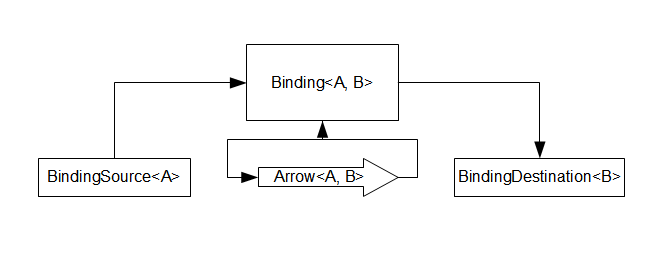
\includegraphics[scale=0.7]{Binding.png}
			\caption{The binding setup}
			%\label{fig\alpha:structural_view}
		\end{figure}
		
		However, there are a number of possible variations on this and so the final approach may differ slightly if a better one is found.
	
	\subsection*{Arrows}
		Arrows will be defined as objects containing C$\sharp$ lambda functions, with an `execute' function which takes an input of the correct type and returns the result of the lambda function applied to it. This will be called by the Binding object which owns the arrow whenever an update to the bound variable is received. Arrow objects will take the input and output types as type parameters, and so the combinators will need to use some form of reflection to dynamically combine arrows of different types which will only be known at runtime. Establishing how exactly to implement this will likely form a significant portion of the initial implementation work. Further to this, allowing arrows to take pairs as inputs (which could potentially be pairs of pairs) will require some form of tree-structured generic type to be developed as an arrow input type.
	
	\subsection*{Invertible Arrows}
		Currently, two possible approaches to implementing invertible arrows are known. One possibility is to require the user to provide both a `set' and a `get' arrow for the binding source (with the assumption being that they will be inverses of each other). The binding would then simply use the `get' when passing a change forward from source to destination, and `set' when passing back.
		
		Another possibility is to limit the range of possible functions to those which are known to be invertible. That is, a set of `basic' arrows would be provided (ideally Turing complete) and the programmer would then build up their desired invertible functions by combining these using the arrow combinators.
		
		The viability of each approach will be explored over the course of the project in order to determine which is the best option, and the reasoning will be discussed in the evaluation.
	
	\subsection*{Possible Extensions}
		There are a number of possible extensions to the project which will be worked on once the main framework is complete:
		
		\begin{itemize}
			\item Unfortunately, C$\sharp$ does not allow the programmer to create custom operators. This means that a Haskell-like syntax for arrows is not possible in the C$\sharp$ implementation. However, the Roslyn framework allows direct access to C$\sharp$'s parser, and allows the programmer to manipulate the result of parsing. This could potentially be used to extend the C$\sharp$ syntax to allow for more natural arrow construction and combination.
			
			\item In a similar vein to the above, the strictness of C$\sharp$'s type system means that the system will make heavy use of generics, and so programmer code will likely have to be littered with type parameters. The goal of this extension would be to minimise these wherever possible, most likely by making liberal use of reflection to derive types.
			
			\item A side-effect of the above is that using reflection to derive types at runtime will most likely have a significant impact on type safety, and potentially lead to runtime type errors and bad conversions where the programmer has made typing mistakes. To make the framework more useful, a good extension would involve adding type checks to the code to ensure that incorrect types aren't being used and throw type exceptions where mistakes are found.
			
			\item Arrows as originally defined by Hughes\cite{hughes98} must conform to a series of `arrow laws'. These are outlined and discussed in detail by Lindley et al\cite{lindley08}. Invertible arrows may well introduce new laws or require modification of the existing ones, and so an extension to the project would be to explore these and derive a new set of laws for invertible arrows.
			
			\item The PostSharp\cite{postsharp} framework allows the programmer to define custom attributes and intercept variables being set and read. This could be used to simplify the creation of binding sources, as the programmer implementing the source could simply place a `Bindable' attribute above the variable they want to bind to and I could set up an Aspect which would handle the generation of events whenever they assigned to the variable.
			
			\item Another possible use of the Roslyn framework for simplifying syntax would be to allow pair arguments to arrows to be passed using simple (v1, v2) syntax rather than by creating a new pair object first.
		\end{itemize}

\section*{Success Criteria}
	The goal of the project is to implement a C$\sharp$ library for one- and two-way data binding, using an implementation of Haskell arrows with special `invertible arrows' for two-way binding. To evaluate the end result, a number of techniques will be used:
	
	\begin{itemize}
		\item As mentioned earlier, C$\sharp$ already has a working data binding system. Thus, a good way of evaluating the implementation would be writing some application which uses data binding non-trivially\footnote{One possible application would be a simple demo in which the user can drag around four line end-points and the point of intersection is automatically drawn. This would be implemented with arrows by having point values in the model which are bound to those in the view by an invertible arrow which translates screen co-ordinates to real co-ordinates, and then a binding from the points in the model to the point of intersection on the screen by an arrow which takes two lines defined as point tuples and outputs the point of intersection.} and comparing the code required by normal data binding and by FRP-based binding for readability, simplicity and elegance.
		
		\item It could also make sense to compare the C$\sharp$ implementation with Haskell arrows (on similar metrics), as a large portion of the work will involve trying to minimise the messy type parameter syntax which will be required to implement general arrow combinators in C$\sharp$.
		
		\item As Hughes' original definition of arrows requires them to follow a set of laws, a successful C$\sharp$ implementation would naturally require that these laws are followed, and so part of the evaluation will consist of verifying this. The main approach for this will be automated testing on random data, but an extension to this would be to attempt a form of semi-formal verification using a simplified mathematical model of the program syntax to prove equalities.
		
		\item Tying in with the third point in `Possible Extensions', if the laws for invertible arrows differ from the standard arrow laws it would also be necessary to test that these are also upheld.
		
		\item It may also make sense to compare the performance of the resulting data binding framework with equivalent bindings expressed in standard .NET binding, though this will effectively be an extension to the evaluation as it will involve working out how exactly to go about this.
	\end{itemize}

\section*{Work plan}
	
	The core implementation work consists of nine work packages. There are then four extension sections, and three for evaluation, with the remaining time allocated to writing the dissertation and fixing any bugs and problems which arise.
	
	\noindent \textbf{Core work packages:}
	
	\subsection*{Work package 1 (22nd October, one week)}
		\begin{itemize}
			\item Setting up Git, backup, C$\sharp$ projects, log etc.
			\item Establishing overall system structure
		\end{itemize}
	
	\subsection*{Work package 2 (29th October, two weeks)}
		Simple demos to test key functionality:
		\begin{itemize}
			\item Get basic (combinator-free) arrows working for arbitrary types
			\item Make a function to combine two arbitrary lambda expressions. Will involve investigating how best to do this, eg. converting into expression trees first, or perhaps storing as expression trees the whole time?
			\item Investigate minimising type parameters
		\end{itemize}
	
	\subsection*{Work package 3 (12th November, two weeks)}
		More simple demos and tests:
		\begin{itemize}
			\item Get a simple two-way binding working and establish the general approach and semantics
			\item Investigate invertible arrows (combinators, implementation techniques etc.) -- may well involve several small demos
		\end{itemize}
	
	\noindent \textbf{Milestone: Various working demos of framework functionality complete}
	
	\subsection*{Work package 4 (26th November, two weeks)}
		\begin{itemize}
			\item Implement the basic binding framework
			\item Implement basic arrows (still combinator-free and probably using lots of type parameters)
		\end{itemize}
	
	\subsection*{Work package 5 (3rd December, one week)}
		\begin{itemize}
			\item Arrow combinators -- get all the standard ones working, probably with type parameters for now
		\end{itemize}
	
	\noindent \textbf{Milestone: Primitive version of the framework is functional}
	
	\subsection*{Work package 6 (10th December, two weeks)}
		\begin{itemize}
			\item Eliminate as many type parameters as possible from arrow combinators using reflection, ExpressionTree constructs etc. -- will require some research into possibilities
		\end{itemize}
	
	\subsection*{Work package 7 (24th December, two weeks)}
		\begin{itemize}
			\item Implement two-way binding
		\end{itemize}
	
	\subsection*{Work package 8 (7th January, two weeks)}
		\begin{itemize}
			\item Investigate and implement invertible arrows (including combinators)
		\end{itemize}
	
	\subsection*{Work package 9 (21st January, one week)}
		\begin{itemize}
			\item Pair arguments -- implement a generic tree-structured arrow argument type to allow for pairs (and pairs of pairs etc.) to be passed as input arguments to arrows
			\item Write progress report
		\end{itemize}
	
	\noindent \textbf{Milestone: Core project is complete, progress report is underway}
	
	\noindent \textbf{Extension work packages:}
	
	\subsection*{Work package 10 (28th January, one week)}
		\begin{itemize}
			\item Complete and submit progress report
			\item Continue work on simplifying syntax -- removing type parameters, making operations more natural etc.
		\end{itemize}
	
	\subsection*{Work package 11 (4th February, one week)}
		\begin{itemize}
			\item Explore possible changes to the arrow laws for invertible arrows
			\item Implement more careful type-checking for generic and reflective code to restore type safety
		\end{itemize}
	
	\subsection*{Work package 12 (11th February, one week)}
		\begin{itemize}
			\item Investigate Rosalyn framework; attempt various small demos
		\end{itemize}
	
	\subsection*{Work package 13 (18th February, one week)}
		\begin{itemize}
			\item Work on simplifying syntax for arrow creation and combination, using Rosalyn or otherwise
			\item Work on simplifying syntax for pair creation
		\end{itemize}
	
	\noindent \textbf{Milestone: End of time allocated for extension work -- as many as time allows will have been implemented}
	
	\noindent \textbf{Evaluation work packages:}
	
	\subsection*{Work package 14 (25th February, two weeks)}
		\begin{itemize}
			\item Evaluate syntax -- compare with Haskell and standard .NET binding via sample apps
			\item Start dissertation
		\end{itemize}
	
		
	\subsection*{Work package 15 (11th March, two weeks)}
		Evaluate arrow laws
		\begin{itemize}
			\item Implement and run automated testing
			\item Attempt to construct a simplified mathematical model and use to prove some of the equalities
			\item Continue work on dissertation
		\end{itemize}

	
	\subsection*{Work package 16 (25th March, one week)}
		(This one will be an extension.)
		\begin{itemize}
			\item Performance comparison between FRP-based data binding and standard .NET equivalent for some non-trivial purpose
			\item Continue work on dissertation
		\end{itemize}
	
	\noindent \textbf{Milestone: Evaluation work complete, dissertation well underway}
	
	\noindent Time left from this point will be allocated to writing the dissertation and fixing any bugs.

\section*{Resource Declaration}

	I will be using my own laptop for the project, or in the event of failure the MCS machines available in the Computer Laboratory. I will ensure all data is backed up online -- code will be hosted on Github, and other data will be hosted elsewhere. In the event of one of these sites going down I will also ensure I have a copy of the entire project on a USB drive.

\clearpage

\begin{thebibliography}{9}

	\bibitem{elliott98}
	Conal Elliott,
	\emph{Composing Reactive Animations},
	1998
	
	\bibitem{haskellarrows}
	Ross Paterson,
	\emph{Arrows: A General Interface to Computation}
	retrieved 08/10/2012
	
	\bibitem{hughes98}
	John Hughes,
	\emph{Generalising Monads to Arrows},
	1998
	
	\bibitem{lindley08}
	Sam Lindley, Philip Wadler, Jeremy Yallop,
	\emph{The Arrow Calculus (Functional Pearl)},
	2008
	
	\bibitem{netbinding}
	MSDN,
	\emph{Data Binding Overview},
	retrieved 08/10/2012
	
	\bibitem{javabinding}
	Greg Weber,
	\emph{Javascript Frameworks and Data Binding},
	2012
	
	\bibitem{paterson03}
	Ross Paterson,
	\emph{Arrows and Computation},
	The Fun of Programming,
	2003
	
	\bibitem{notifypropertychanged}
	MSDN,
	\emph{INotifyPropertyChanged Interface},
	retrieved 08/10/2012
	
	\bibitem{postsharp}
	Code Project,
	\emph{Aspect Oriented Programming using C$\sharp$ and PostSharp},
	retrieved 17/10/2012

\end{thebibliography}

%\end{document}